%=====================================================================
% CISP-BMEI 2026 submission
% Track: CISP -- Signal Modeling, Identification & Prediction
%
% Compile with the official CISP-BMEI LaTeX template on Overleaf.
% This file uses IEEEtran conference class, which the CISP-BMEI template is based on.
% NOTE: no LaTeX toolchain is available on the machine where this was authored, so this
% source has NOT been compiled locally. It is written to be compiled on Overleaf.
%=====================================================================
\documentclass[conference]{IEEEtran}
\IEEEoverridecommandlockouts

\usepackage{cite}
\usepackage{amsmath,amssymb,amsfonts}
\usepackage{algorithmic}
\usepackage{graphicx}
\usepackage{textcomp}
\usepackage{xcolor}
\usepackage{booktabs}
\usepackage{url}
\usepackage{tikz}
\usetikzlibrary{arrows.meta,positioning,calc}

\graphicspath{{../figures/}}

% This paper carries five floats in six pages, which is float-heavy for IEEEtran. The default
% placement fractions (topfraction 0.7, textfraction 0.2) force floats onto separate pages and
% leave text pages half-empty; relaxing them packs the floats alongside the text.
\renewcommand{\topfraction}{0.92}
\renewcommand{\bottomfraction}{0.85}
\renewcommand{\textfraction}{0.06}
\renewcommand{\floatpagefraction}{0.75}
\setcounter{topnumber}{3}
\setcounter{bottomnumber}{2}
\setcounter{totalnumber}{5}

% Tighten the vertical spacing that display math, lists and floats consume. The paper has
% seven display equations, a seven-item list and four floats; the default skips add up to
% roughly a third of a page across the document, and none of it is content.
\setlength{\abovedisplayskip}{3pt plus 1pt minus 1pt}
\setlength{\belowdisplayskip}{3pt plus 1pt minus 1pt}
\setlength{\abovedisplayshortskip}{2pt plus 1pt}
\setlength{\belowdisplayshortskip}{2pt plus 1pt}
\setlength{\textfloatsep}{7pt plus 2pt minus 2pt}
\setlength{\floatsep}{7pt plus 2pt minus 2pt}
\setlength{\intextsep}{7pt plus 2pt minus 2pt}
\setlength{\abovecaptionskip}{4pt plus 1pt minus 1pt}
\setlength{\belowcaptionskip}{2pt plus 1pt minus 1pt}

\def\BibTeX{{\rm B\kern-.05em{\sc i\kern-.025em b}\kern-.08em
    T\kern-.1667em\lower.7ex\hbox{E}\kern-.125emX}}

% Placeholders that must be replaced with measured values before submission.
\newcommand{\TBD}[1]{\textcolor{red}{[#1]}}

\begin{document}

\title{Neural or Classical Solvers for the HJB Equation of Optimal\\ Execution? A Closed-Form Comparison and a\\ Decision Guide}

\author{
\IEEEauthorblockN{Jingwen Zhang}
\IEEEauthorblockA{\textit{School of Mathematics and Physics} \\
\textit{Xi'an Jiaotong-Liverpool University}\\
Suzhou, China}
\and
\IEEEauthorblockN{Fei Ma}
\IEEEauthorblockA{\textit{School of Mathematics and Physics} \\
\textit{Xi'an Jiaotong-Liverpool University}\\
Suzhou, China}
}

\maketitle

\begin{abstract}
Physics-informed neural networks (PINNs) are widely proposed for optimal-control problems in
finance on the grounds of the curse of dimensionality, but for the
Hamilton--Jacobi--Bellman equation of optimal execution it is unclear \emph{when} a neural solver
is the right choice and when a classical one is. We compare three classical schemes (explicit
finite differences and Howard policy iteration, with the grid variants they imply) and two neural
ones (a direct PINN and a policy-iteration PINN) on a multi-asset optimal-execution HJB whose value
function has a closed-form matrix Riccati solution. The analytic reference removes a circularity
common in this literature --- one solver serving as the accuracy reference for the others, and so
reporting zero error by construction --- and it stays exact at every state dimension, which lets us
measure accuracy where no classical baseline can be run at all.

The comparison yields a boundary rather than a winner. Where a grid scheme can run ($p \le 5$) it
is both faster and more accurate, by a factor of $5$ to $50$ in time at $p=4$--$5$ and by two to
three orders of magnitude at low dimension. Beyond $p \approx 5$ it is not runnable at the
resolution the accuracy target needs, and the mesh-free solver is the only method that runs, at
accuracy decaying from $R^2 = 0.98$ at $p=8$ to $0.76$ at $p=20$ with no internal signal of the
decay.

Two results explain why the usual framing misleads. An HJB is solved so that it can be acted on,
and the control is a \emph{derivative} of the value function: with the multilinear reconstruction
standard in this setting the control error is 13 to 185 times the value error, whereas a cubic
reconstruction on the same nodes is four to five orders of magnitude more accurate and brings the
ratio to 2.8. Value accuracy therefore does not bound control accuracy, and a benchmark reporting
only the former measures the wrong quantity. Second, the neural solver's failure is a property of
\emph{parameterisation}, not dimension: at the same dimension, architecture and budget a separable
problem fails catastrophically ($R^2 = -688$ at $p=8$) where a non-separable one is solved well
($0.981$).

We close with the decision the comparison supports: a grid scheme for a single instance at low
dimension, a neural solver where the dimension makes the grid infeasible, and a learned operator
--- which amortises after roughly $10^3$ parameter settings --- when a family of problems must be
solved rather than one.
\end{abstract}

\begin{IEEEkeywords}
Hamilton--Jacobi--Bellman equation, physics-informed neural networks, neural operators, optimal
execution, high-frequency trading, numerical methods, solver benchmarking, curse of
dimensionality, method selection, reproducibility, out-of-domain extrapolation.
\end{IEEEkeywords}

%=====================================================================
\section{Introduction}
%=====================================================================

Deep learning methods for partial differential equations (PDEs) are frequently proposed for
optimal control in finance on the grounds that mesh-based solvers suffer from the curse of
dimensionality. In high-frequency trading (HFT), the relevant control problem is the
Hamilton--Jacobi--Bellman (HJB) equation of optimal execution or market making, with state
variables such as mid-price, inventory, volatility and spread. The natural question is
therefore practical rather than rhetorical: given such a problem, should it be solved with a neural
solver or a classical one, and does the answer change with dimension? This paper answers that by
running both on the same problem and scoring both against an answer that is known exactly.

The comparison is worth making carefully, for three reasons. Much of the applied literature scores
a solver against \emph{another solver}, which makes the reference exact by construction and its
reported error zero; a closed-form solution removes that circularity. Most comparisons also report
one accuracy number, the value function, when the quantity an HJB is solved for is the control ---
a derivative, obtained differently by each family, and as it turns out not equally accurately.
And most are run in a single regime, whereas the answer here depends on the regime, so a comparison
that does not vary dimension and deployment model cannot support a recommendation.

This paper makes six contributions.

\textbf{(1) A closed-form comparison.} We cast multi-asset optimal execution
as a linear--quadratic (LQ) HJB problem whose value function is available in closed form from
a matrix Riccati equation, and we solve it with four methods that differ in how they obtain a
control. Having an analytic reference matters for two reasons. First, it
makes accuracy meaningful. Much of the applied literature measures a solver's error against
another numerical method, and whichever method serves as the reference is then exact by
construction and reports zero error, which is circular. Second, the LQ structure yields the
optimal control in closed
form, $u^\star = -R^{-1}B^\top P(t)x$, which turns the sign convention of the control law
into something that can be tested rather than assumed. The same Riccati solution reduces to
the classical Almgren--Chriss inventory trajectory in the forced-liquidation limit, which we
use as an independent check.

Some recent frameworks solve high-order PDEs by replacing nested automatic differentiation with
explicit matrix recursions. SHoP \cite{xiao2024shop} is a recent example, proposed for exactly
this HFT setting. The claim worth testing is not whether such derivatives can be computed, but
whether the resulting solver is competitive with classical schemes at the dimensions this problem
actually has.

\textbf{(2) Value accuracy is not control accuracy.} The
control is the deliverable of an HJB and is a \emph{derivative} of the value function, so a grid
scheme must differentiate an interpolant while a network differentiates itself exactly. We show
that the two errors decouple, and then locate the cause: placing the exact closed-form value
function on the grid, so the solution carries no error, reproduces essentially the whole control
error, which means the grid solution is not the limiting factor. We measure three reconstructions
on functions with known gradients. A multilinear interpolation is second order; taking instead its
exact gradient is also second order --- so consistency with the interpolant buys nothing --- and a
cubic reconstruction is fourth order on non-polynomial functions and four to five orders of
magnitude more accurate on the same nodes. On the benchmark's own solved grid the cubic
extraction cuts the control/value error ratio from 185 to 2.8. Time refinement cannot substitute
for a better reconstruction. The consequence is that the resolution an application needs is set by the control
target \emph{and} by the order of the differentiation operator, and that value accuracy --- the
quantity benchmarks report --- bounds neither.

\textbf{(3) A comparison across the axis that decides the answer.} We measure value-function and
control accuracy and solve time for explicit finite differences, Howard policy iteration and a PINN,
from $p=1$ to $p=20$, with multiple seeds for the stochastic solver. Grid methods require $N^p$
points, and their time step is limited by the Courant--Friedrichs--Lewy (CFL) condition on the mesh
spacing, so work grows faster than $N^p$ as $p$ rises. We therefore ran a separate grid-refinement
study to find the resolution each $p$ needs to reach a fixed accuracy target, so that the
comparison is accuracy-matched rather than resolution-matched, and a training-budget study, because
a fixed-budget comparison would understate the neural solver; a larger budget did recover the
accuracy a smaller one lost, and we report that rather than the version that flattered the grid
method. The result is a boundary rather than a winner. Where the grid scheme can run at all
($p \le 5$) it is both faster and more accurate. Beyond that ($p \ge 8$) the mesh-free solver is
the only method that runs, at accuracy decaying from $R^2 = 0.98$ at $p=8$ to $0.76$ at $p=20$
while its control-sign agreement stays near $0.7$, so nothing in the method itself warns the user
that it is deteriorating.

\textbf{(4) A failure mode that depends on parameterisation, not dimension.} Extending the sweep
required abandoning the symmetric parameterisation it started with, because with uniform
coefficients the value function is exactly separable and the sweep was not testing the
curse of dimensionality at all. On a genuinely non-separable problem the PINN does not collapse.
More pointedly, at the \emph{same} dimension, architecture and budget, a separable problem fails
catastrophically ($R^2 = -688$ at $p=8$) while a non-separable one is solved well
($R^2 = 0.981$). A permutation-symmetric problem appears to be the harder optimisation target for
a generic multilayer perceptron (MLP). The practical consequence is narrow and testable: do not
validate a PINN for this
class of equation on a symmetric toy problem, because success there is not evidence about the
general case --- and, as we found, failure there is not evidence against it either.

\textbf{(5) A decision guide.} The comparison supports a recommendation, which we state as a table
mapping each regime --- single instance or parameter family, low dimension or high, accuracy
critical or not --- to the method that the measurements favour and the measurement that decides it.
We also record the two ways a neural solver fails that a user will not see from inside: its
accuracy decays with dimension without any internal signal, and it is sensitive to how the problem
is parameterised rather than to how hard the problem is.

\textbf{(6) A cautionary case of out-of-domain evaluation.} We reproduce a failure mode first
encountered in a released HFT implementation. We evaluated a network trained on a normalised price
domain ($[20,30]$, terminal target 25) on raw asset prices from 40 to 550,
with the volatility and spread channels also outside their training ranges. Measuring the
model's \emph{local} price sensitivity $|\partial V/\partial S|$ --- threshold-free, unlike the
no-trade fraction, which depends on an arbitrary rule --- shows it falls monotonically with
price level, by a factor of about 54 across the nine instruments, with a rank correlation of
$-0.90$ to $-1.00$ over three seeds. The network saturates further outside its training
domain, so its response to price is suppressed in proportion to how far the instrument sits
from that domain. Any threshold applied to this gradient inherits the ordering, which produces
a cross-sectional ``finding'' --- typically that the model prefers not to trade high-priced,
liquid instruments --- that admits a plausible microstructure story while being entirely an
artefact of scale. Mapping the input back into the training domain removes the dependence
(rank correlation $+0.12$, $-0.22$, $+0.23$). Out-of-domain failure of learned PDE operators is
known; what we add is its \emph{shape} in a control setting --- saturation rather than divergence,
so the damage survives every sanity check that looks for obviously broken output and instead
appears as a clean cross-sectional ranking.

Section~\ref{sec:bench} defines the benchmark and its analytic solution.
Section~\ref{sec:defects} catalogues the defects we found in the baseline implementation and
the ablation design used to quantify them. Section~\ref{sec:setup} gives the experimental
setup, Section~\ref{sec:results} the results and Section~\ref{sec:disc} discusses scope and
limitations.

%=====================================================================
\section{Related Work}
%=====================================================================

Avellaneda and Stoikov derived closed-form approximations for market-making control under
inventory risk \cite{avellaneda2008high}; Gu\'eant \emph{et al.} formulated optimal execution
under market impact as a nonlinear HJB problem \cite{gueant2013dealing}; Cartea and Jaimungal
added risk criteria and microstructure features \cite{cartea2015risk,cartea2015algorithmic}; and
Almgren and Chriss gave the canonical mean--variance trajectory \cite{almgren2000optimal}, which
is the forced-liquidation limit of our benchmark. Classical numerical treatments include
Markov-chain approximation \cite{kushner1990numerical}, monotone finite-difference schemes
\cite{forsyth2017epsilon} and policy iteration \cite{howard1960dynamic,bertsekas2012dynamic};
these are accurate and well understood but scale poorly in the number of state variables.

On the neural side, PINNs embed the PDE residual in the loss \cite{raissi2019physics}, alongside
the deep Galerkin and deep Ritz methods \cite{sirignano2018dgm,yu2018deep} and deep BSDE solvers
\cite{han2018solving,e2017deep}. For the HJB specifically, the strongest precedents for
\emph{scale} are mesh-free and single-instance: the deep Galerkin method reached a
21-dimensional HJB, and a penalty formulation of the coupled HJB--continuity system solved
mean-field games in 100 dimensions on a workstation \cite{carmona2020machine}. Those results are
arguments for mesh-free representation, which we do not dispute; they are not cost comparisons
against a classical solver, which is what we supply here.
High-order derivatives are the recognised bottleneck, because
nested reverse-mode differentiation grows quickly in memory and time
\cite{hutzenthaler2022overcoming}; explicit matrix recursions such as SHoP \cite{xiao2024shop}
are one response. Domain decomposition and adaptive refinement reduce training cost
\cite{meng2020ppinn,moseley2021finite}.

Learned solution \emph{operators} are the more recent line: FNO \cite{li2021fourier,li2023neural},
CNO \cite{raonic2023convolutional}, Transolver \cite{wu2024transolver} and others map function
spaces rather than solving one instance, so a single trained model serves a family of problems.
Two features of that literature matter for this paper. First, its cost claims are framed at
\emph{inference} time, and that framing is legitimate rather than a strawman: the classical
baseline must be re-solved for every new instance. FNO states this directly --- ``the optimization
problem needs to be solved for every new instance'' while ``the neural operator needs to be
trained only once'' --- and UGrid concedes it from the other side, noting that when only the
right-hand side changes and the classical solver's setup cost is already amortised, the classical
method wins \cite{han2024ugrid}. Second, benchmark work reports training
and inference cost as separate metrics rather than one number \cite{pdenneval2024}, which is why
this paper reports both. What the operator literature does \emph{not} contain, in the corpus we
examined, is any application to HJB, optimal control or Bellman equations: every HJB paper we
found is single-instance and non-operator. The gap this paper addresses is narrower and more
specific than ``neural methods for PDEs'' --- it is the absence of an accuracy-matched,
closed-form-referenced cost comparison for the HJB at HFT-relevant dimensions.

Applications to pricing and portfolio problems are established, but applications to \emph{HFT} ---
where the state dimension is modest and latency requirements are severe --- are
underexplored, which is the gap we examine quantitatively.

Two pitfalls recur in this literature. First, circular validation: one solver serves as the ground
truth for the others, which is common when no analytic solution is available. Second, evaluating
neural surrogates outside their training distribution is a well-documented failure mode in machine
learning. What we add is a concrete, quantitative
instance in a financial control problem, where the resulting artefact is smooth, monotone and
therefore unusually easy to rationalise.

%=====================================================================
\section{Benchmark Problem and Analytic Reference}\label{sec:bench}
%=====================================================================

\subsection{Multi-asset optimal execution in LQ form}
Let $x \in \mathbb{R}^p$ denote inventory in $p$ assets and $u \in \mathbb{R}^p$ the trading
rate, with linear dynamics and additive noise,
\begin{equation}
dx = (Ax + Bu)\,dt + \Sigma\,dW .
\end{equation}
The trader maximises expected risk-adjusted proceeds,
\begin{equation}
\sup_{u}\ \mathbb{E}\!\left[
-\tfrac{1}{2}\!\int_0^T\!\!\big(x^\top Q x + u^\top R u\big)dt
-\tfrac{1}{2}x_T^\top Q_T x_T
\right],
\end{equation}
where $u^\top R u$ is temporary market impact ($R = \eta I$), $x^\top Q x$ is an inventory
risk penalty ($Q = \lambda\sigma^2 I$), and the terminal term penalises residual inventory.
This is the Almgren--Chriss problem in LQ form; with $A = 0$, $B = I$ it reproduces the
classical trajectory. The HJB equation is
\begin{equation}
\begin{split}
-\partial_t V = \max_u\Big\{-\tfrac{1}{2}\big(x^\top Qx + u^\top Ru\big)
+ (\nabla V)^\top(Ax + Bu)\Big\} \\
+ \tfrac{1}{2}\mathrm{tr}\big(\Sigma\Sigma^\top \nabla^2 V\big),
\end{split}
\end{equation}
with $V(x,T) = -\tfrac{1}{2}x^\top Q_T x$.

\subsection{Closed-form solution}
Substituting the quadratic ansatz $V(x,t) = -\tfrac{1}{2}x^\top P(t)x + c(t)$ gives the
matrix Riccati equation and an additive constant,
\begin{align}
-\dot P &= Q + PA + A^\top P - PBR^{-1}B^\top P, \qquad P(T) = Q_T, \\
\dot c &= \tfrac{1}{2}\,\mathrm{tr}\big(\Sigma\Sigma^\top P\big), \qquad c(T) = 0,
\end{align}
and the optimal control
\begin{equation}\label{eq:ustar}
u^\star(x,t) = -R^{-1}B^\top P(t)\,x .
\end{equation}
Eq.~\eqref{eq:ustar} is what makes the sign convention testable: for a liquidation problem
with $q > 0$ and $P(t) \succeq 0$, the optimal rate is \emph{negative}. A solver that returns
the positive of this quantity is inverted, and any backtest built on it trades the wrong way
in every period.

For the scalar case the Riccati solution has the closed form
\begin{equation}
P(t) = \eta k\,\frac{Q_T\cosh\!\big(k(T{-}t)\big) + \eta k\sinh\!\big(k(T{-}t)\big)}
{\eta k\cosh\!\big(k(T{-}t)\big) + Q_T\sinh\!\big(k(T{-}t)\big)},
\end{equation}
with $k=\sqrt{Q/\eta}$; as $Q_T \to \infty$, $P(t)$ tends to $\eta k\coth(k(T-t))$, and in that
limit the optimal trajectory is the classical
$q_t = q_0\sinh(k(T-t))/\sinh(kT)$. We use both limits as independent checks on the
reference implementation (Section~\ref{sec:setup}).

\subsection{Why this benchmark}
Four properties make this a fair test: the value function and control are analytic, so accuracy
and sign are falsifiable; the dimension $p$ is free, so the curse-of-dimensionality claim can be
measured rather than asserted; the structure matches the HFT HJB used in practice (drift,
diffusion, quadratic running cost, control penalty, terminal penalty), so it is a legitimate
relaxation rather than a toy; and every method solves the same equation, with the Hamiltonian
maximisation applied identically, so the comparison isolates representation and discretisation.

%=====================================================================
\section{Defects in the Baseline Implementation}\label{sec:defects}
%=====================================================================

Before benchmarking, we audited a released HFT-HJB implementation whose results we set out to
reproduce. The audit found eight distinct defects, seven of which we ablate individually (D3
and D4 live in the same expression and cannot be separated). Several are generic rather than
specific to that codebase, which is why we list them.

\begin{itemize}\itemsep1pt
\item[\textbf{D1}] \emph{Ordering.} Minute CSVs were stored newest-first and never sorted, so the
``previous'' bar in every lag was the \emph{next} minute. The summed price return in file order is
$+0.037950$ against $-0.021709$ in chronological order: the reported P\&L has the wrong sign.
\item[\textbf{D2}] \emph{Same-bar leak.} Position came from bar $i$'s close and was multiplied by
a return spanning that same bar, so the strategy saw the move it was trading.
\item[\textbf{D3/D4}] \emph{Control law.} The control was hard-coded as $-\nabla V/(2\kappa)$ in
three places --- the negative of the HJB first-order condition Eq.~\eqref{eq:ustar} --- and it also
dropped the $1/(2\kappa S)$ factor, where $\kappa$ and $S$ are the baseline's impact and price
parameters. Every minute classified as a buy signal (19.1\% of the sample)
has a negative trading rate, a strict pointwise inversion rather than a partial bias.
\item[\textbf{D5}] \emph{Position vs.\ rate.} Position was set to the trading rate rather than its
integral, although the model specifies that position is the integral of the trading rate,
$dx = u\,dt$; the ``position'' is dimensionless and unrelated to inventory.
\item[\textbf{D6}] \emph{Cost units.} Costs were computed in currency units and subtracted from a
return series, so they exceed gross P\&L by orders of magnitude and the result measures the cost
model rather than the signal.
\item[\textbf{D7}] \emph{Annualisation.} Minute returns were annualised with
$(1+r)^{252/N_{\text{min}}}$ and $\mathrm{sd}\cdot\sqrt{252}$, mixing a minute-level series with
daily factors; the reported volatilities and Sharpe ratios are not interpretable.
\item[\textbf{D8}] \emph{Input scaling.} The network was trained on a price domain of $[20,30]$
and evaluated on raw prices of 40 to 550 (Section~\ref{sec:ood}).
\end{itemize}

Two further issues concern the pipeline rather than the accounting: features were computed
non-causally (log returns used \texttt{shift(1)} on a newest-first file; VWAP was a global
cumulative sum), and the ``spread'' input was the high--low range, which cannot be a bid--ask
spread since the source provides only OHLCV bars. Our corrected pipeline sorts ascending before
any lagged computation, accumulates VWAP forward from the sample start, and replaces the range
with a published effective-spread estimator (Section~\ref{sec:setup}).

%=====================================================================
\section{Methodology}\label{sec:setup}
%=====================================================================

\subsection{Overview}
Figure~\ref{fig:method} shows the design. We pose a problem whose answer is known in closed form,
solve it with four methods that differ in \emph{how they obtain a control}, and score every solver
on both the value function and the control against that answer. The design turns the usual
benchmark question --- which method is more accurate --- into two sharper ones: accuracy in
\emph{which} quantity, and at what cost in dimension.

\input{fig_method.tex}

The four methods fall into two families on the one axis this paper is about. A grid solver stores
$V$ at $N^p$ nodes and must \emph{reconstruct} a continuous function from them before it can
differentiate one; a network \emph{is} a continuous function, so automatic differentiation returns
its gradient exactly. Everything the paper reports about control accuracy follows from that
difference, and from the order of the reconstruction the grid solver uses.

\subsection{Reference implementation checks}
We validated the analytic reference against three independent closed forms: the
finite-$Q_T$ Riccati solution, the $Q_T\to\infty$ limit (which recovers $\eta k\coth(k(T-t))$), and
the classical Almgren--Chriss inventory trajectory in the same limit. Measured maximum errors
were $9.8\times10^{-12}$, $1.0\times10^{-9}$ and $4.3\times10^{-9}$ respectively, and the
control law matched $u^\star=-P(t)q/\eta$ to $8.9\times10^{-16}$. The control sign was verified
negative for positive inventory across all sampled states.

\subsection{Problem parameters}
We use well-scaled defaults: $\eta = 0.01$, $\lambda\sigma^2 = 0.01$, $Q_T = 0.1$,
$\sigma = 0.01$, $T=1$, giving $k=1$. These keep the control magnitude $O(1)$-$O(10)$ so that
the explicit time step is set by a realistic CFL bound rather than by an artificial stiffness.

\subsection{Solvers}
\textbf{The finite-difference scheme} uses explicit backward time stepping on a tensor-product grid of
$N$ points per dimension, with the analytic Hamiltonian maximiser and central differences in
space. \textbf{Policy iteration} uses Howard's algorithm on the same grid: policy evaluation
solves the linear frozen-policy PDE and policy improvement sets $u = R^{-1}B^\top\nabla V$. Two
implementation points matter. First, because the frozen-policy term is genuine advection, the
evaluation step must be upwinded: central differencing of a frozen advection term is
unconditionally unstable, and it diverged in our first implementation. Second, the policy is
stored as a function of $(x,t)$: the optimal policy here is $u^\star(x,t)=-R^{-1}B^\top P(t)x$
with strongly time-dependent $P(t)$, and collapsing it to a single time-independent array made
the evaluation PDE inconsistent near $t=T$.

\subsection{The physics-informed neural network}
A PINN represents the solution as a network and trains it to satisfy the PDE itself, so no
solution data are needed. Here the network $\mathcal{N}$ maps $(x,t)\mapsto V$ and is trained by
minimising the HJB residual

\begin{equation}
\begin{split}
r(x,t) \;=\; & \frac{\partial V}{\partial t} \;+\; \frac{1}{2}\sigma^{2}\Delta V
   \;-\; \tfrac12\big(x^\top Q x + u^{\star\top} R u^{\star}\big) \\
   & \;+\; \big(\nabla V\big)^\top\!\big(Ax + Bu^{\star}\big),
\end{split}
\end{equation}

with $u^{\star}=R^{-1}B^\top\nabla V$ substituted analytically, so the supremum over the control
never has to be learned and the residual is a function of $\nabla V$ and $\Delta V$ alone. Three
design choices carry the accuracy and are stated here because they are what a reader must know to
judge the later comparisons.

\emph{The terminal condition is imposed exactly, not as a penalty.} We write

\begin{equation}
V(x,t) \;=\; V_T(x) \;+\; (T-t)\,\mathcal{N}(x,t),
\end{equation}

where $V_T(x)=V(x,T)$ is the known terminal payoff. Then $V(x,T)=V_T(x)$ for \emph{any} network
parameters, so the terminal condition contributes no error and no penalty weight has to be tuned
against the residual. This matters more here than in a forward PDE, because the terminal region is
where the control is largest.

\emph{The residual is normalised, and collocation is biased towards the terminal time.} The
residual is divided by its value at initialisation so the loss starts at $O(1)$ and the same
learning rate works at every dimension $p$. Collocation points are drawn with a density
proportional to $(1-u)^{\beta}$ in time ($u\sim U(0,1)$, $\beta=3$), concentrating samples near
$t=T$, where $|\nabla V|$ --- and hence $|u^\star|$ --- is largest; uniform sampling leaves that
region under-resolved.

\emph{Inputs are scaled by an explicit component.} The state box is mapped affinely to $[-1,1]$
and time to $[0,1]$. This is not cosmetic: it is the component whose omission produces the
out-of-domain failure documented in Section~\ref{sec:ood}, so it is treated as part of the model
rather than as preprocessing.

The architecture is a $4\times64$ $\tanh$ MLP, trained with Adam. \emph{No architecture search is
performed}, so every neural statement in this paper is a claim about a competently trained
standard PINN, not about the best achievable network; Section~\ref{sec:disc} returns to this.

\subsection{The accuracy protocol}
All accuracy metrics are computed against the analytic solution, never against another solver, and
are averaged over several time slices so a method that ignores the time dimension cannot score
well. Two quantities are reported separately --- the value function and the control --- because
they turn out not to agree, which is the subject of Section~\ref{sec:control}. For the grid
methods the control depends on how the value function is reconstructed before it is
differentiated, so three reconstructions are compared in Section~\ref{sec:control}: a
piecewise-linear (multilinear) one probed by finite differences, that same reconstruction
differentiated exactly, and a cubic one probed identically.

\subsection{Data, splitting and preprocessing}
Experiments with real data use minute bars for nine US instruments (AAPL, AMZN, GOOGL, MSFT,
NVDA, OXY, QQQ, SPY, TSLA). The two shipped windows (2025-03-06 to 2025-04-04 and 2025-03-27
to 2025-04-25) overlap only on 2025-03-27 to 2025-04-04. We use a strictly temporal split in
which training and test share no dates: training 2025-03-06 to 03-26, validation 03-27 to
04-04, test 04-07 to 04-25. Preprocessing sorts ascending before computing log returns and
EWMA volatility, accumulates VWAP forward and replaces the high--low range with the Roll
effective-spread estimator \cite{roll1984simple}, cross-checked against
Corwin--Schultz \cite{corwin2012simple}; the implied spreads
(1.2--7.0\,bp across these names) are consistent with known effective spreads, whereas the
daily Corwin--Schultz estimate is upward biased here.

\subsection{Hardware}
All neural training and all reported timings run on a single NVIDIA RTX 4090 Laptop GPU
(17.2\,GB). Grid-method timings run on the CPU. We state the timing methodology explicitly
because CPU-only neural timings are not comparable to compiled grid solvers, and because the
comparison is a central claim.

%=====================================================================
\section{Results}\label{sec:results}
%=====================================================================

\subsection{Accuracy and cost against the analytic solution}
\input{tables/tab_main.tex}

Table~\ref{tab:main} is the central result. The finite-difference scheme is the most accurate
method at every dimension, with value $R^2$ between $0.99927$ and $0.99999$, and its control has
the correct sign at every sampled state. Policy iteration converges in 13 outer iterations and is
slightly less accurate ($R^2 = 0.9908$ to $0.9966$), as expected from the first-order upwind
discretisation used in its policy-evaluation step.

We had to reduce the grid resolution as $p$ grew, so comparing cost at the resolutions the sweep
could afford would be unfair. A separate refinement study therefore swept $N$ at
each $p$ and found the smallest resolution reaching a fixed accuracy target of $R^2 \ge 0.9999$.
That resolution is $N^\star = 21$ at \emph{every} dimension tested, which gives one
accuracy-matched grid configuration per $p$; the grid columns of Table~\ref{tab:main} use it.
Grid cost grows far faster than the point count $N^p$ by itself would suggest, because the explicit time
step is CFL-limited by the mesh spacing and work scales closer to $N^{p+1}$: at $p=5$, $N=21$ is
$4.1\times10^6$ points over 420 steps, which is why accuracy-matched finite differences cost
nearly 15 minutes at a dimension the neural solver covered in under four.

At matched accuracy the grid scheme is faster than the fixed-budget neural solver at every
dimension: by a factor of 5.6 at $p=4$ and by two to three orders of magnitude at $p \le 2$. The
mesh-free solver's cost is indeed almost flat in $p$ ($95 \rightarrow 226$\,s, a factor of $2.4$
across five dimensions) against $0.023 \rightarrow 865$\,s for the grid scheme, so the two curves
do cross --- but at the crossing the neural solver is no longer solving the problem.

The PINN's accuracy is competitive at low dimension ($R^2 = 0.9997 \pm 0.0002$ at $p=1$) and
degrades with $p$, failing outright at $p \ge 4$ under this budget. A negative $R^2$ means the
learned value function is worse than predicting the mean, so the method has not solved the
problem rather than merely lost accuracy. Note that control-sign agreement stays high even where
$R^2$ is negative: the network recovers the \emph{direction} of the optimal control while missing
its level. Sign agreement alone is therefore not evidence that an HJB solver works. It is the sort
of diagnostic that is easy to report and easy to over-read, so it should not stand in for one.

\emph{That failure is specific to this parameterisation, not to the dimension} --- see
Section~\ref{sec:highdim}, where a non-separable version of the same problem at the same
dimensions is solved successfully while the separable version fails catastrophically. We flag it
here rather than leaving the table to speak for itself.

\subsection{Value accuracy is not control accuracy}\label{sec:control}

The comparison above is in the currency this literature normally uses: the value function. But an
HJB is solved so that it can be \emph{acted on}, and what is acted on is the optimal control
$u^\star = -R^{-1}B^\top \nabla V$ --- a \emph{derivative} of the value function. A grid scheme
must obtain that derivative in two steps: reconstruct the stored nodal values as a continuous
interpolant, then differentiate it. A network obtains it in one, by automatic
differentiation, which is exact for whatever function the network represents. We call the first
step the \emph{reconstruction}, and its \emph{order} is the degree of the local polynomial piece
it uses: one for a piecewise-linear (multilinear) reconstruction, three for a cubic one. A
reconstruction of order $k$ yields a gradient that converges at a rate set by $k$, and it is that
rate --- not the accuracy of the solved value function --- that governs the control error. The two
steps together we call the \emph{extraction}. The value and control errors need not be
accurate to the same degree. If they are not, then reporting value accuracy alone answers a
question nobody asked.

They are not, and the reason is more specific --- and more fixable --- than the observation that
derivatives are hard to estimate. Table~\ref{tab:control} reports both errors against the same
closed-form reference, on the same solutions. At every dimension and every resolution tested the
control error exceeds the value error, and it converges at a stable order of approximately $2.00$:
least-squares fits of $\log(\text{error})$ against $\log h$ give $2.00$, $1.96$, $1.96$, $1.96$
and $1.96$ at $p = 1,\dots,5$, with fit $R^2$ between $0.998$ and $1.000$. The value error
converges faster on average but irregularly, and at the finest grid in two of the five dimensions
it regresses, so the ratio between the two grows under refinement --- at $p=2$ it runs
$2 \to 5 \to 13 \to 25 \to 49 \to 83 \to 179$ over $N = 11,\dots,61$ --- until the value error
stops behaving.

\emph{The cause is the reconstruction, not the solution.} To separate the two we put the
closed-form value function on the grid as exact nodal values, so the discrete solution is
error-free by construction and every remaining control error belongs to the step that turns nodal
values into a gradient. With the multilinear interpolation and probing difference used above that
step alone reproduces almost all of it --- $3.7\times10^{-3}$ against $3.8\times10^{-3}$ at $N=11$,
falling to
$1.1\times10^{-4}$ at $N=61$, at order $1.98$, against $3.8\times10^{-3} \to 1.1\times10^{-4}$
measured on the solved grid. The grid solution is not what limits control accuracy.

\emph{What limits it is the order of the reconstruction.} Replacing the probing difference on a
multilinear interpolant with the same probing difference on a cubic one --- which is $C^2$, so its
gradient is smooth rather than piecewise constant --- changes the error by four to five orders of
magnitude on the same grid. Table~\ref{tab:extract} measures this on functions whose gradients are
known exactly, so the orders are properties of the reconstruction rather than of this benchmark.
The multilinear reconstruction is second order on every function tested; taking instead the
\emph{exact} gradient of that same interpolant, which is the best a piecewise-linear
reconstruction can do, is also second order, so consistency with the interpolant buys nothing. The
cubic reconstruction is fourth order and better on the non-polynomial functions and exact on the
quadratic one. Because this benchmark's value function \emph{is} quadratic, the last column of that
table applies the same comparison to the Merton problem, whose closed form is a power function and
whose HJB is non-linear in the derivatives; there the cubic order is $5.2$ against $2.1$.

\input{tables/tab_extract.tex}

This is why value accuracy and control accuracy can be chosen almost independently. On the
benchmark's own solved grid at $p=2$, $N=61$, the multilinear extraction gives a control error of
$1.1\times10^{-4}$ against a value error of $6.1\times10^{-7}$, a ratio of 185. The cubic
extraction gives $1.7\times10^{-6}$ on the same grid --- a factor of 67 better --- and there the
control error is set by the solver rather than by the reconstruction, so the ratio falls to $2.8$.
The decoupling reported above is therefore largely an artefact of the gradient operator chosen, not
a property of grid methods.

\input{tables/tab_control.tex}

\emph{Refining in time cannot substitute for any of this.} Holding the mesh fixed and varying only
the number of stored snapshots --- refining in time and nothing else --- separates the two errors
cleanly. The value error falls by two to four orders of magnitude ($\times23$, $\times163$,
$\times428$ at $p=2$ for $N=21,35,45$; $\times4{,}559$, $\times17{,}269$, $\times4{,}249$ at
$p=3$). The control error falls by only $\times3.8$, $\times10$, $\times17$ at $p=2$, and then
stops improving; at $p=5$ it does not improve at all ($\times1.0$). The value error is
\emph{time}-limited; the control error is limited by the reconstruction. The plateau the control
error settles at is not arbitrary: at $p=2$ it scales as $h^2$ to within measurement error --- from
$1.005\times10^{-3}$ at $h=0.125$, $O(h^2)$ predicts $3.48\times10^{-4}$ and $2.07\times10^{-4}$
at $h = 0.0735$ and $0.0568$, against measured $3.46\times10^{-4}$ and $2.10\times10^{-4}$, a
discrepancy of 0.5\% and 1.4\%.

An unintended experiment makes the same point from the opposite direction. At $p=5$, moving from
$N=15$ to $N=17$ refined the mesh, but a memory cap in our own solver silently halved the
snapshot count from 41 to 20, coarsening time. The control error \emph{improved}
($1.999\times10^{-3} \to 1.780\times10^{-3}$, matching the $O(h^2)$ prediction), while the value
error \emph{degraded} ($2.135\times10^{-4} \to 9.207\times10^{-4}$). The two errors moved in
opposite directions because the two refinements did. Raising the cap restored the value error to
$1.120\times10^{-4}$ --- a factor of 8.2 --- and with it the monotone growth of the ratio, from
$3 \to 4 \to 9 \to 9 \to 2 \to 1$ back to $3 \to 5 \to 7 \to 9 \to 15 \to 23$ on the same grids.
We report this because it is an easy trap to fall into and a hard one to notice: any automatic,
memory-driven reduction of stored time levels changes the quantity that controls value accuracy,
and the resulting error looks spatial.

\emph{The lever is the reconstruction, not the grid.} This reverses the practical advice that
follows from the comparison above. Value accuracy can be bought with time resolution, whose
storage cost is linear in the number of stored levels; control accuracy, for the reconstruction
used here, could only be bought with spatial resolution, whose cost is $N^p$ --- which is the
curse of dimensionality appearing as a consequence of the control target rather than the value
target. But the reconstruction order is a third axis, orthogonal to both, and moving along it
costs nothing at the grid level: a cubic reconstruction on the \emph{same} nodes delivers four to
five orders of magnitude. The resolution an HJB application needs is therefore not fixed by the
control target alone; it is fixed by the control target \emph{and} the order of the operator used
to differentiate the solution. A benchmark that reports only value accuracy, and a solver whose
control is a probing difference on a multilinear interpolant, will both understate what is
achievable and misattribute the cost.

\emph{This is not an argument that control error is harmless.} The envelope theorem cuts the other
way for value: because the value function is stationary at the optimum, a control error $\delta u$
perturbs the optimal \emph{value} only by $O(\|\delta u\|^2)$, so a control error of $10^{-3}$ can
move the value by $10^{-6}$ and be invisible in value terms. That is an argument for measuring the
error on the executed path, not for ignoring it. What an implementation executes is $u$, and the
inventory path is a time integral of the control and therefore inherits the control error to \emph{first}
order. A solver can therefore be accurate enough for valuation, which is what a value-accuracy
benchmark certifies, and still execute the wrong inventory. A backtest that reuses the same
control will not reveal the error. At the boundaries this is worse rather than better: inside a
no-trade region, or against an inventory constraint, stationarity does not apply and the error is
first order in both quantities. The claim we make is the narrow, safe one: value accuracy does
not bound control accuracy, so a benchmark must report the quantity the application actually
uses.

Two caveats we do not paper over. First, the value error's own convergence is irregular (orders of
1.6 to 5.6, and non-monotone at the finest grids), whereas the control order is stable at 2.00 ---
which is what one expects if the value error is not a clean spatial quantity but a mixture of time
discretisation, snapshot placement and mesh error. Second, this benchmark's value function is
quadratic and a cubic reconstruction reproduces quadratics \emph{exactly}, so the
machine-precision result above is a best case; the quotable numbers are the fourth-order
convergence and the four to five orders of magnitude on non-polynomial functions.

That second caveat is the one a referee should press on, so we tested it directly rather than
leaving it open. The Merton portfolio problem has a closed-form solution that is a \emph{power}
function, $V(x,t) = (x^\gamma/\gamma)e^{\kappa(T-t)}$, and an HJB that is genuinely non-linear in
the derivatives --- the maximised term is a ratio of a squared first derivative to a second
derivative. Two things follow. The cubic reconstruction is no longer exact, and its measured order
on that value function is $5.2$ against the multilinear reconstruction's $2.1$ (Table
\ref{tab:extract}, last column). Second, when we solve the Merton HJB numerically and run the same
comparison is run on the solved grid, the cubic extraction is $959\times$ more accurate at
$N=321$ (order $3.91$ against $2.04$) and is by then tracking the solver's own error rather than
the reconstruction's. The result is therefore not an artefact of the linear--quadratic structure,
which was the remaining way it could have been.

\subsection{Does the neural solver hold up as the dimension grows?}\label{sec:highdim}

The sweep above stops at $p=5$ because grid methods stop being runnable past that. The analytic
reference does not: the Riccati equation is $p^2$ ODEs whatever $p$ is, so accuracy can still be
\emph{measured} at dimensions where no classical baseline can be run. We extended the range to
$p=20$ to test the dimensionality claim directly.

Doing so exposed a flaw in the sweep above. With the uniform defaults
($Q=\lambda\sigma^2 I$, $R=\eta I$, $A=0$) the value function is \emph{separable}:
$V(x,t)=\sum_i v(x_i,t)$ for a single scalar $v$. Solving that at $p=20$ is barely harder than at
$p=1$, because the network only has to apply one learned univariate function and sum. That is not
the case the curse-of-dimensionality argument is about, so we added per-asset heterogeneity ---
each asset draws its own risk aversion and impact coefficient, and the off-diagonal terms of $Q$
are random, so $V$ becomes a $p$-dimensional quadratic with a full $P$ matrix. We
re-validated the reference implementation on this problem up to $p=20$ ($P$ symmetric and positive
definite, terminal condition exact, control sign correct for positive inventory).

\input{tables/tab_highdim.tex}

The result is not what the separable sweep would have predicted. On the non-separable problem the
PINN does not collapse; it degrades with dimension, giving $R^2 = 0.99999$, $0.9994$,
$0.9992$, $0.977$, $0.981$, $0.927$ and $0.757$ at $p = 1$, $2$, $3$, $5$, $8$, $12$ and $20$. A
grid baseline remains available and more accurate through $p=5$ (0.9999 down to
0.9993) but is not runnable at $p \ge 8$, where $N^p$ alone is $2\times10^7$ points before the
CFL-limited time step is counted. Beyond that point the mesh-free solver is the only method that
runs at all --- at accuracy that declines to $0.76$ by $p=20$ and that the user cannot bound,
because nothing is left to compare against except the analytic solution we happen to have
here.

The separability control is the sharpest single result. At $p=8$, the \emph{separable} problem
fails catastrophically ($R^2 = -688$) while the non-separable, harder problem is solved
well ($R^2 = 0.981$). The earlier failure is therefore a property of that parameterisation, not of
the dimension: a permutation-symmetric problem appears to be a harder optimisation target for a
generic MLP than a heterogeneous one, presumably because the symmetric case has degenerate
directions and a much weaker training signal. We had no prior expectation of this and report it as
found. It also means the practical guidance is narrower than ``PINNs fail at high dimension'': what
fails is a specific combination of architecture, parameterisation and budget, and the same
architecture succeeds at the same dimension once the problem is made generic.

The honest reading of the dimension study is therefore three-part. Grid methods are the better tool
wherever they are runnable, which is up to about $p=5$ at the resolutions needed for $10^{-4}$
accuracy. The neural solver is the only option beyond that, and it does produce usable
approximations to $p \approx 12$. But its accuracy decays without any internal signal that it is
decaying --- the control-sign agreement stays near $0.7$ even at $p=20$ where $R^2 = 0.76$ --- so
deployment at those dimensions would need the analytic or high-accuracy reference that this
benchmark supplies and that a real problem would not.

One objection to that reading is under-training, and it deserves a direct answer. Scaling the
training budget along two
axes gives the following (mean over seeds; a single seed where noted). At $p=4$ the fixed
budget of 6000 epochs and 2048 collocation points yields $R^2 = -44.5$ in 177\,s; 20000 epochs
at the same batch yields $R^2 = +0.9972$ in 630\,s. At $p=3$ the same increase moves $R^2$ from
$0.9981$ (two seeds, min $0.9970$) in 172\,s to $0.9997$ in 541\,s. The failure in
Table~\ref{tab:main} is therefore a statement about budget, not about capacity, and we say so
rather than presenting the fixed-budget comparison as a verdict on the method.

What does not change is the cost. The rescued $p=4$ run took 630\,s against 31.7\,s for
accuracy-matched finite differences at the same dimension --- about $20\times$ more expensive,
for lower accuracy ($R^2 = 0.9972$ versus $0.99991$). Since the neural solver's cost grows only
slowly in $p$ while the grid scheme's grows geometrically, the gap must close eventually; over
$p = 1$ to $5$ it does not close, and at each dimension where both methods succeed the grid
scheme is faster by a factor of $5$ to $50$.

A second result is less expected: increasing the collocation count at a fixed number of steps
does not substitute for more steps. Quadrupling the batch to 8192 while holding epochs at 6000
pushed $p=4$ from $-44.5$ to $-310$ and $p=3$ from $0.9981$ to $0.9860$. More samples per step
made the optimiser \emph{worse} within the same step budget, because each step's averaged
gradient is noisier in the higher-dimensional residual and the learning-rate schedule is
exhausted before convergence. Practitioners tuning a PINN on this problem class should scale the
step count, not the batch.

\begin{figure}[t]
\centering
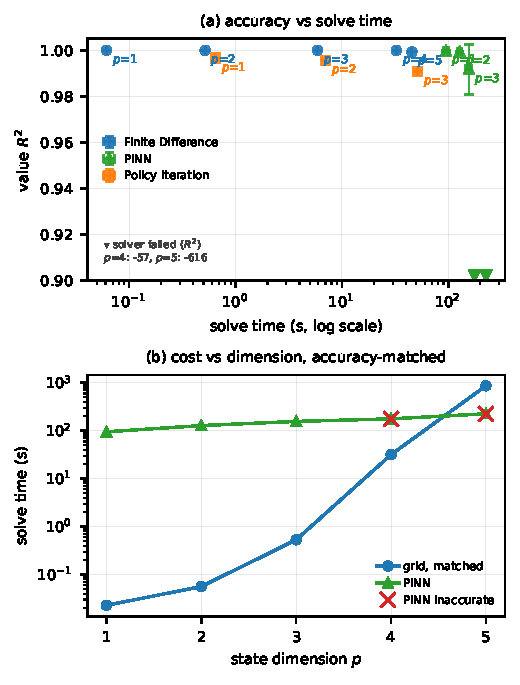
\includegraphics[width=\columnwidth]{fig1_accuracy_and_cost.pdf}
\caption{Left: value-function accuracy against wall-clock solve time for every method and
dimension; up and to the left is better. The neural solver's $p=4$ and $p=5$ runs have negative
$R^2$ and are pinned to the axis floor. Right: solve time against state dimension at equal
accuracy. Grid cost grows geometrically in $p$; the mesh-free solver's does not.}
\label{fig:acc}
\end{figure}

\subsection{Out-of-domain evaluation as a spurious-signal generator}\label{sec:ood}

To isolate the mechanism we train the baseline's style of network --- a $4\times64$ $\tanh$ MLP
taking (price, volatility, spread, time), on the HJB residual with a soft terminal condition
$V(S,T) = -\tfrac{1}{2}(S-25)^2$ --- on prices sampled from $[20,30]$ only. We then evaluate it
on the realised price levels of the instruments, which range from \$42 to \$536.

Fig.~\ref{fig:ood} reports the magnitude of the learned price sensitivity
$|\partial V/\partial S|$ at those prices. Under raw-price evaluation it falls monotonically with
price --- from $3.36$ at \$42, through $0.573$ at \$154 and $0.359$ at \$202, to $0.062$ at
\$536, a factor of about 54 --- with rank correlations of $-0.90$, $-0.98$ and $-1.00$ across
three seeds. The interpretation is direct: the network saturates in proportion to how far its
input lies beyond the training domain, so its responsiveness to price is suppressed exactly for
the high-priced instruments. This is a property of the input scaling, not of the market.

We measure the sensitivity rather than the no-trade fraction deliberately. The no-trade fraction
is a thresholded function of this gradient, so it inherits the ordering, but its levels depend on
the threshold --- and the audited baseline used two mutually inconsistent rules for that
threshold. The monotone dependence on price level is the invariant; the particular fractions are
not.

Applying the correction --- an affine map of the evaluation prices back into $[20,30]$, with
the returned gradient converted to true price units by the chain rule --- removes the
dependence: the rank correlations become $+0.12$, $-0.22$ and $+0.23$, scattered around zero,
and $|\partial V/\partial S|$ no longer spans the factor-of-54 range across instruments. The
sensitivity to the correction is itself the diagnostic: the artefact shows up as an ordering that
tracks an input's scale.

\begin{figure}[t]
\centering
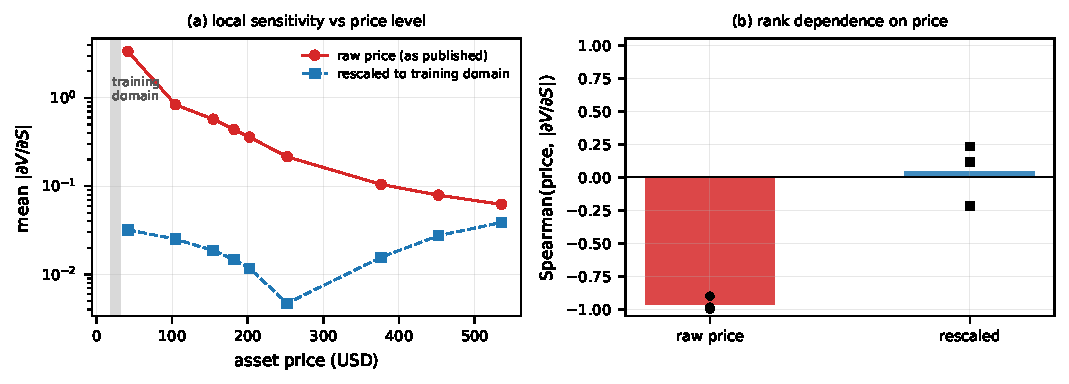
\includegraphics[width=\columnwidth]{fig3_ood_no_trade.pdf}
\caption{Out-of-domain artefact and its removal. (a) Mean $|\partial V/\partial S|$ against
instrument price level; the shaded band is the training domain. Raw-price evaluation produces
a monotone decay of roughly 54$\times$ as the network saturates outside the domain. (b) Rank
correlation between price level and sensitivity, per seed, for both treatments.}
\label{fig:ood}
\end{figure}

\subsection{Contribution of each defect}
\input{tables/tab_ablation.tex}

Table~\ref{tab:ablation} fixes each accounting defect in isolation, on the out-of-sample
window, and averages over nine instruments and three seeds. Two defects dominate, and they move
the headline numbers in different ways.
Fixing the chronological ordering (D1) flips the sign of the reported return, from $-7.9\%$ to
$+1.3\%$: as noted in Section~\ref{sec:defects}, the summed price return in file order has the
opposite sign to the true one, so the as-published P\&L is inverted relative to the actual
strategy. Fixing the annualisation (D7) leaves the return untouched --- it is an accounting
identity on the return series --- but changes the reported volatility by a factor of about 25,
from $3.7\%$ to $91.6\%$. That single defect is why the Sharpe ratios in the as-published
configuration ($-0.14$) cannot be read as risk-adjusted performance: the number is a function of
the annualisation convention, not of the strategy. Adopting the HJB control law (D3/D4) improves
the return to $-4.2\%$, cuts turnover from $3.3$ to $3.0$ and, because the corrected control is
bounded by the spread threshold rather than by an arbitrary clip, reduces gross exposure from
$|q| = 1.00$ to $0.71$ --- but it does not on its own flip the sign.

Fixing the input scaling (D8) in isolation makes the performance \emph{worse} ($-93.0\%$),
which is the expected consequence of repairing one defect while the others remain: once the
network actually responds to price, the still-inverted control law and the non-integrated
position produce extreme positions --- turnover rises from $3.3$ to $57.6$ --- and the costs
follow. This is a useful reminder that defect ablation is not a decomposition into independent
contributions; only the joint correction is interpretable.

With all defects fixed the out-of-sample result is a total return of $+1.1\%$ and a Sharpe
ratio of $+0.34$ over the test window. We deliberately make no performance claim from this. The
test window is 14 trading days, on which no Sharpe ratio is statistically distinguishable from
zero, and the point estimate is unstable across the single-defect corrections, ranging from
$-93\%$ to $+1.3\%$. What the table does establish is that the as-published figures were driven
by accounting choices rather than by a property of the strategy: the same model on the same data
supports $-7.9\%$ or $+1.3\%$ depending only on whether the bars are sorted, and a Sharpe ratio
of $-0.14$ or $-1.20$ depending only on how returns are annualised.

% The defect-ablation figure is omitted: Table~\ref{tab:ablation} carries the same numbers more
% precisely, and a full-width three-panel figure costs about half a page that the six-page
% budget does not have.

%=====================================================================
\section{Discussion and Limitations}\label{sec:disc}
%=====================================================================

\subsection{When to use which}
Table~\ref{tab:guide} states the recommendation the comparison supports. Every row is a regime a
practitioner can recognise before committing to a method, and every recommendation points at a
measurement in this paper rather than at a preference.

\input{tables/tab_guide.tex}

Two features of that table are worth drawing out, because they are the opposite of how the choice
is usually framed. First, the neural solver is preferred in only two rows, and in both the reason
is that the classical scheme cannot be run or should not be re-run --- not that it was beaten on
accuracy. Where the two can be compared, the classical scheme wins on both axes. Second, the
largest single improvement available to a grid user is not a finer grid but a better
reconstruction: four to five orders of magnitude on the same nodes, at no cost in dimension. A
practitioner who takes only that one line from this paper will have gained more than the choice of
solver would have given them.

\subsection{Scope of the benchmark}
The LQ problem is a relaxation of the market-making HJB: it
keeps inventory, quadratic impact, transaction costs and a terminal penalty, but it is
linear--quadratic, and the optimal control is state-feedback in inventory and time. A trader
with no alpha should indeed trade only to manage inventory, so this is economically natural,
but the benchmark does not exercise price-predictive signals, order-book features, limit
orders or the non-quadratic impact and latent-liquidity effects that appear at short
horizons. Conclusions about \emph{relative solver cost and accuracy} transfer; conclusions
about achievable P\&L do not, and we make none.

\textbf{Training time versus inference time.} A natural objection is that the comparison should
use inference time, not training time, on the grounds that a trained network evaluates in
microseconds while a numerical scheme must be re-solved. We measured both, and the objection
does not hold here, but the reason is precise and worth setting out, because the reasoning is not
specific to this problem.

Neither method is ``solve long'' versus ``evaluate fast''. Both have the same structure:
an expensive offline solve followed by cheap online queries. The grid scheme's offline cost is
the sweep of Table~\ref{tab:main}; its online cost is multilinear interpolation of the stored
snapshot. Amortised over a batch of 390 states --- one trading day of minute decisions --- the
per-state control evaluation costs 0.66\,$\mu$s at $p=1$, 5.07\,$\mu$s at $p=3$ and
34.3\,$\mu$s at $p=5$ for the grid scheme, against 3.0--4.9\,$\mu$s for the PINN on GPU at the
same dimensions. The neural solver's inference is therefore \emph{not} uniformly faster: at $p=1$ the
grid interpolation is about $4.5\times$ quicker than a forward pass plus autograd, because
interpolating a small table is cheaper than evaluating a network. The PINN's inference wins only
as $p$ grows, where multi-dimensional interpolation degrades and the network's cost does not.

The right way to combine the two components is the total cost of $N$ evaluations,
$T(N) = T_{\text{offline}} + N\,t_{\text{eval}}$, and to ask where it breaks even. At $p=1$ the
PINN never does: the grid scheme is cheaper both upfront ($0.023$\,s against $95$\,s) and per
evaluation. At $p=3$ the PINN's inference is faster (3.60 against 5.07\,$\mu$s) but repaying its
156\,s training cost takes $1.1\times10^{8}$ evaluations, or about $270{,}000$ trading days at
390 decisions per day. At $p=5$ the neural solver is finally cheaper on \emph{both} terms ---
$226$\,s of training against an $865$\,s solve, and $4.9$ against $34.3$\,$\mu$s per query ---
which is precisely the curse-of-dimensionality argument; the reason it does not win in practice
is that at that dimension it is not accurate ($R^2 = -616$). The binding constraint has moved
from cost to accuracy.

That analysis holds for \emph{one} HJB. The operator literature works in a different regime, and
the two regimes must be separated explicitly, because both are correct and they have opposite
answers. In the many-instance regime, where a classical solver must be re-solved for every member
of a family of problems, the comparison is
$M\,T_{\text{solve}}$ against $M_{\text{data}}T_{\text{solve}} + T_{\text{train}} + M\,t_{\text{infer}}$,
where the data term charges the operator for the classical solutions it is trained on. Solving for
the break-even instance count $M^\star$ with a training set of $10^3$ classical solves gives
$4{,}365$ instances at $p=2$, $1{,}383$ at $p=3$, $1{,}024$ at $p=4$ and $1{,}000$ at $p=5$ ---
essentially the size of the training set, because once $t_{\text{solve}} \gg t_{\text{infer}}$ the
second sweep is nearly free. An operator therefore amortises after $1{,}000$ to $4{,}365$ parameter settings,
and the threshold \emph{falls} as dimension rises. A calibration or robustness study spanning
thousands of parameter combinations is exactly such a family, and for those the neural route is
the right one. Our benchmark is a single instance, which is why it reports the other answer.

The objection would therefore be decisive under a per-query re-solve model --- say, model
predictive control whose parameters change every step. But a fixed-parameter PINN does not escape
that either: it learned $P(t)$ for one parameter set, so changed parameters mean retraining.
Exploiting the regime properly requires an \emph{operator} that takes the model parameters as
inputs and amortises one training run across many settings. That is a different method,
and we regard it as the most promising direction this benchmark points to.

Two obstacles to that direction come from the operator literature rather than from us. Most
operator architectures are trained on paired input--output data, so for
the HJB they would need labelled solutions from the classical solver they aim to replace --- the
$M_{\text{data}}T_{\text{solve}}$ term above is not incidental. The exception is the
physics-informed operator family \cite{wang2021physics}, which trains on the PDE residual and
needs no labels, and it is therefore the most natural fit here, but it has been demonstrated on
forward PDEs in one and two dimensions and, as far as we can determine, never on an HJB with a
supremum over controls. Spectral operators carry a specific hazard for this problem too: the
value function $V$ is convex but not periodic, so truncating a Fourier basis aliases exactly at
the inventory boundaries where the optimal control switches between buying, holding and selling.
A pragmatic route, and the one we would pursue, is two-stage: solve the HJB with a mesh-free
method at the dimensions where that is affordable, then distil the solutions into a
parameter-conditioned operator that can be queried across a parameter family.

Neural training is timed on a GPU and grid solves on a CPU, which flatters the neural method; we
state that rather than adjust for it, and the ordering holds under either convention.

A further detail is worth reporting because it cuts against the usual intuition. For a
\emph{single} state rather than a batch, the PINN is faster on the CPU than on the GPU --- 0.31
to 0.92\,ms against 1.14 to 2.74\,ms --- because one evaluation is dominated by kernel launch
overhead rather than arithmetic. A GPU is the wrong tool for one decision at a time, and
batching, not raw throughput, is what makes it competitive. We report the evaluation costs
rather than leaving them implied, because for a reader deciding what to deploy, solve time and
run-time latency are different questions with different answers.

\textbf{The out-of-domain lesson is not specific to finance.} The mechanism --- smooth,
monotone, apparently meaningful structure produced by extrapolation in one input channel ---
applies to any surrogate trained on a normalised domain and evaluated on physical units. It is
also not a new phenomenon in general terms: out-of-domain failure of learned PDE operators, and
the unreliability of their uncertainty estimates when an input parameter leaves the training
range, are documented and addressed in the operator literature
\cite{chandra2024uncertainty}. Our contribution is not the existence of the failure but its
\emph{shape} in a control setting: because the network saturates rather than diverging, its price
sensitivity decays smoothly and monotonically, so the damage survives every sanity check that
looks for obviously broken output and instead appears as a clean cross-sectional ranking. Our
recommendation is procedural: report per-channel input coverage for every evaluation set, and
treat any cross-sectional result whose ordering coincides with an input's scale as suspect
until input scaling has been ruled out.\footnote{We do not reproduce the six numerical claims
in the audited baseline that could not be traced to any code path; they are excluded from
this paper.}

\textbf{Limitations.} (i) The grid scheme is not runnable beyond $p \approx 5$ at the resolution the
accuracy target needs, so the comparison becomes accuracy-only there; we still report it, because
a practitioner at $p=20$ faces exactly that situation, but the cost half of the argument stops at
$p=5$. (ii) The neural results use one architecture ($4\times64$ $\tanh$), one optimiser and one
learning-rate schedule, and we do not perform an architecture search; every neural claim here is a
statement about a competently trained standard PINN. Techniques designed for high-dimensional PDEs
--- domain decomposition \cite{meng2020ppinn,moseley2021finite}, adaptive collocation, or
architectures that build in the quadratic structure --- could plausibly shift where the boundary
sits, and we release the benchmark precisely so that such claims can be tested against a
closed-form reference rather than against another numerical method. (iii) The separability effect
is established as a phenomenon, not explained: we show that a symmetric problem fails where a
non-separable one succeeds at the same dimension, architecture and budget, but we have not
established the mechanism, and we do not claim that symmetry \emph{causes} the failure.
(iv) Real-data results use nine instruments over a two-month window, so they characterise the
pipeline's behaviour rather than the strategy's expected profitability. (v) Timings come from a
single GPU and CPU, so absolute values are hardware-specific; the comparison is stated as
GPU-for-neural
versus CPU-for-grid, which favours the neural method and therefore does not weaken the negative
conclusion. (vi) The control-accuracy result is established for this family of schemes: a
second-order explicit grid solver whose control is a finite difference of an interpolated value
function. Higher-order spatial reconstruction, or a scheme that solves for the control directly
rather than differentiating the value function, could narrow the gap, and we have not tested
them; what we have shown is that the gap is not closed by refining in time, which is the cheap
direction.

%=====================================================================
\section{Conclusion}
%=====================================================================

We compared neural and classical solvers for the HJB equation of multi-asset optimal execution,
against a closed-form Riccati reference, in order to answer a question a practitioner actually
faces: which one to use. The comparison does not produce a winner, and the reason it does not is
the paper's main finding. The two families are not ranked along one axis but along three, and the
axis that decides the answer is not the one usually reported.

Measuring the value function --- which is what this literature measures --- says classical methods
win. Measuring the \emph{control}, which is what an HJB is for,
says something different: the two errors decouple, the control error is the larger of the two, and
it is not improved by refining in time. The tempting conclusion is that control accuracy can only
be bought with spatial resolution, at cost $N^p$ --- the curse of dimensionality reappearing as a
consequence of the control target. That conclusion is wrong, and locating the error is the point of
this paper. Putting the exact value function on the grid, so the solution carries no error at all,
reproduces essentially the whole control error; the grid solution is not the limiting factor. What
limits it is the order of the operator that turns nodal values into a gradient. A multilinear
reconstruction is second order; taking its exact gradient is also second order; and a cubic
reconstruction on the same nodes is fourth order and four to five orders of magnitude more
accurate, which brings the control error down to the solver's own level and cuts the control/value
error ratio from 185 to 2.8.

The resolution an application needs is therefore set by the control target \emph{and} by the order of the
differentiation operator --- and the second of those is free. Value accuracy cannot reveal this,
because it does not bound control accuracy. We would report the control error, the order of the
reconstruction and the input-domain coverage alongside any value-accuracy figure.

Within the range where a grid scheme can run --- up to about five state dimensions at the
resolution the value target demands --- it is also both faster and more accurate, by a factor of
roughly $5$--$50$ in time at $p=4$--$5$ and by two to three orders of magnitude at low dimension.
Beyond that the grid scheme is not merely slow but not runnable, and the mesh-free solver is the only
method that runs, at accuracy decaying from $R^2 = 0.98$ at $p=8$ to $0.76$ at $p=20$ with no
internal signal that it is decaying. Classical methods therefore win wherever the comparison can be
made --- and the regime the dimensionality argument is about, where the neural route is the only
one available, is precisely the regime where this benchmark can only score the neural solver, not
race it.

That is the sense in which there is no winner, and it is why
Table~\ref{tab:guide} is conditional rather than a ranking. The neural solver is preferred in two
of its rows, and in both the reason is that the classical scheme cannot be run or should not be
re-run --- not that it was beaten. A reader who wants one actionable line should take the second
row instead: if control accuracy matters, the cheapest available improvement is not a different
solver, a finer grid or more training, but a higher-order reconstruction of the value function on
the nodes already computed.

We tested the two obvious objections to that reading and both changed the picture without
reversing it. Under-training is real: a larger optimisation budget recovers accuracy a smaller one
loses, and we report the rescued run rather than the flattering comparison. Inference-versus-training
is also real, and the field's preference for inference time is justified, because a classical
solver must be re-solved for every new problem instance. But the two framings answer different
questions --- one problem, or a family of them --- and they have opposite answers: a single HJB
favours the classical scheme, while an operator amortises a parameter family after roughly
$10^3$--$10^4$ instances. Reporting either number without naming the deployment model is what makes
this literature hard to read.

Two methodological results generalise beyond this equation. A surrogate trained on a normalised
state domain and evaluated in physical units fails smoothly rather than loudly: its local
sensitivity decays monotonically with distance from the training range (rank correlation $-0.90$
to $-1.00$ across seeds here), so any threshold applied to it produces cross-sectional structure
that looks economically meaningful while being an artefact of scale. A neural solver's failure
can be a property of the problem's symmetry rather than its dimension: at the same dimension,
architecture and budget, a separable problem failed catastrophically where a non-separable one was
solved well. Both point the same way --- validate on the problem you actually have, with a
reference you can trust, and report the input coverage and the deployment model alongside any cost
claim.

\section*{Reproducibility}
Code, the temporal data splits, the preprocessing manifest and every raw result file behind the
tables and figures are released.\footnote{Repository link to be added.} Solver accuracy is
measured against the analytic reference; the reference itself is checked against three
independent closed forms; and the backtest accounting is covered by unit tests against
hand-computed values. The manuscript is built and page-checked by \texttt{src/build\_paper.py}.

\bibliographystyle{IEEEtran}
\bibliography{refs}

\end{document}
